\documentclass[twoside]{book}

% Packages required by doxygen
\usepackage{fixltx2e}
\usepackage{calc}
\usepackage{doxygen}
\usepackage[export]{adjustbox} % also loads graphicx
\usepackage{graphicx}
\usepackage[utf8]{inputenc}
\usepackage{makeidx}
\usepackage{multicol}
\usepackage{multirow}
\PassOptionsToPackage{warn}{textcomp}
\usepackage{textcomp}
\usepackage[nointegrals]{wasysym}
\usepackage[table]{xcolor}

% Font selection
\usepackage[T1]{fontenc}
\usepackage[scaled=.90]{helvet}
\usepackage{courier}
\usepackage{amssymb}
\usepackage{sectsty}
\renewcommand{\familydefault}{\sfdefault}
\allsectionsfont{%
  \fontseries{bc}\selectfont%
  \color{darkgray}%
}
\renewcommand{\DoxyLabelFont}{%
  \fontseries{bc}\selectfont%
  \color{darkgray}%
}
\newcommand{\+}{\discretionary{\mbox{\scriptsize$\hookleftarrow$}}{}{}}

% Page & text layout
\usepackage{geometry}
\geometry{%
  a4paper,%
  top=2.5cm,%
  bottom=2.5cm,%
  left=2.5cm,%
  right=2.5cm%
}
\tolerance=750
\hfuzz=15pt
\hbadness=750
\setlength{\emergencystretch}{15pt}
\setlength{\parindent}{0cm}
\setlength{\parskip}{3ex plus 2ex minus 2ex}
\makeatletter
\renewcommand{\paragraph}{%
  \@startsection{paragraph}{4}{0ex}{-1.0ex}{1.0ex}{%
    \normalfont\normalsize\bfseries\SS@parafont%
  }%
}
\renewcommand{\subparagraph}{%
  \@startsection{subparagraph}{5}{0ex}{-1.0ex}{1.0ex}{%
    \normalfont\normalsize\bfseries\SS@subparafont%
  }%
}
\makeatother

% Headers & footers
\usepackage{fancyhdr}
\pagestyle{fancyplain}
\fancyhead[LE]{\fancyplain{}{\bfseries\thepage}}
\fancyhead[CE]{\fancyplain{}{}}
\fancyhead[RE]{\fancyplain{}{\bfseries\leftmark}}
\fancyhead[LO]{\fancyplain{}{\bfseries\rightmark}}
\fancyhead[CO]{\fancyplain{}{}}
\fancyhead[RO]{\fancyplain{}{\bfseries\thepage}}
\fancyfoot[LE]{\fancyplain{}{}}
\fancyfoot[CE]{\fancyplain{}{}}
\fancyfoot[RE]{\fancyplain{}{\bfseries\scriptsize Generated by Doxygen }}
\fancyfoot[LO]{\fancyplain{}{\bfseries\scriptsize Generated by Doxygen }}
\fancyfoot[CO]{\fancyplain{}{}}
\fancyfoot[RO]{\fancyplain{}{}}
\renewcommand{\footrulewidth}{0.4pt}
\renewcommand{\chaptermark}[1]{%
  \markboth{#1}{}%
}
\renewcommand{\sectionmark}[1]{%
  \markright{\thesection\ #1}%
}

% Indices & bibliography
\usepackage{natbib}
\usepackage[titles]{tocloft}
\setcounter{tocdepth}{3}
\setcounter{secnumdepth}{5}
\makeindex

% Hyperlinks (required, but should be loaded last)
\usepackage{ifpdf}
\ifpdf
  \usepackage[pdftex,pagebackref=true]{hyperref}
\else
  \usepackage[ps2pdf,pagebackref=true]{hyperref}
\fi
\hypersetup{%
  colorlinks=true,%
  linkcolor=blue,%
  citecolor=blue,%
  unicode%
}

% Custom commands
\newcommand{\clearemptydoublepage}{%
  \newpage{\pagestyle{empty}\cleardoublepage}%
}

\usepackage{caption}
\captionsetup{labelsep=space,justification=centering,font={bf},singlelinecheck=off,skip=4pt,position=top}

%===== C O N T E N T S =====

\begin{document}

% Titlepage & ToC
\hypersetup{pageanchor=false,
             bookmarksnumbered=true,
             pdfencoding=unicode
            }
\pagenumbering{alph}
\begin{titlepage}
\vspace*{7cm}
\begin{center}%
{\Large Pool \\[1ex]\large 1 }\\
\vspace*{1cm}
{\large Generated by Doxygen 1.8.14}\\
\end{center}
\end{titlepage}
\clearemptydoublepage
\pagenumbering{roman}
\tableofcontents
\clearemptydoublepage
\pagenumbering{arabic}
\hypersetup{pageanchor=true}

%--- Begin generated contents ---
\chapter{Namespace Index}
\section{Namespace List}
Here is a list of all documented namespaces with brief descriptions\+:\begin{DoxyCompactList}
\item\contentsline{section}{\mbox{\hyperlink{namespace_ui}{Ui}} \\*This \mbox{\hyperlink{class_dialog}{Dialog}} class is for the visualization of the pool game }{\pageref{namespace_ui}}{}
\end{DoxyCompactList}

\chapter{Hierarchical Index}
\section{Class Hierarchy}
This inheritance list is sorted roughly, but not completely, alphabetically\+:\begin{DoxyCompactList}
\item \contentsline{section}{Ball}{\pageref{class_ball}}{}
\item \contentsline{section}{Ball\+Builder}{\pageref{class_ball_builder}}{}
\begin{DoxyCompactList}
\item \contentsline{section}{concrete\+Ball\+Builder}{\pageref{classconcrete_ball_builder}}{}
\end{DoxyCompactList}
\item \contentsline{section}{Coordinate}{\pageref{class_coordinate}}{}
\item \contentsline{section}{Game\+Factory}{\pageref{class_game_factory}}{}
\begin{DoxyCompactList}
\item \contentsline{section}{Stage1\+Factory}{\pageref{class_stage1_factory}}{}
\end{DoxyCompactList}
\item Q\+Dialog\begin{DoxyCompactList}
\item \contentsline{section}{Dialog}{\pageref{class_dialog}}{}
\end{DoxyCompactList}
\item \contentsline{section}{Table}{\pageref{class_table}}{}
\item \contentsline{section}{Table\+Builder}{\pageref{class_table_builder}}{}
\begin{DoxyCompactList}
\item \contentsline{section}{Concrete\+Table\+Builder}{\pageref{class_concrete_table_builder}}{}
\end{DoxyCompactList}
\end{DoxyCompactList}

\chapter{Class Index}
\section{Class List}
Here are the classes, structs, unions and interfaces with brief descriptions\+:\begin{DoxyCompactList}
\item\contentsline{section}{\mbox{\hyperlink{class_ball}{Ball}} \\*\mbox{\hyperlink{class_ball}{Ball}} class used for store the info of ball json objects. It contains basic setters, getters and methods that detect and resolve wall-\/collison and balls-\/collisons }{\pageref{class_ball}}{}
\item\contentsline{section}{\mbox{\hyperlink{class_ball_builder}{Ball\+Builder}} \\*Ballbuilder class is the abstract builder class for object ball }{\pageref{class_ball_builder}}{}
\item\contentsline{section}{\mbox{\hyperlink{classconcrete_ball_builder}{concrete\+Ball\+Builder}} \\*Concrete\+Ball\+Builder class is the concrete builder class for object ball }{\pageref{classconcrete_ball_builder}}{}
\item\contentsline{section}{\mbox{\hyperlink{class_concrete_table_builder}{Concrete\+Table\+Builder}} \\*\mbox{\hyperlink{class_concrete_table_builder}{Concrete\+Table\+Builder}} class is the concrete builder class for object table }{\pageref{class_concrete_table_builder}}{}
\item\contentsline{section}{\mbox{\hyperlink{class_coordinate}{Coordinate}} \\*\mbox{\hyperlink{class_coordinate}{Coordinate}} class is for ball class to have a convienent way to store its position info }{\pageref{class_coordinate}}{}
\item\contentsline{section}{\mbox{\hyperlink{class_dialog}{Dialog}} }{\pageref{class_dialog}}{}
\item\contentsline{section}{\mbox{\hyperlink{class_game_factory}{Game\+Factory}} \\*This is the abstract factory class in abstract factory method }{\pageref{class_game_factory}}{}
\item\contentsline{section}{\mbox{\hyperlink{class_stage1_factory}{Stage1\+Factory}} \\*This is the concrete factory class in abstract factory method }{\pageref{class_stage1_factory}}{}
\item\contentsline{section}{\mbox{\hyperlink{class_table}{Table}} \\*This is the class for table objects }{\pageref{class_table}}{}
\item\contentsline{section}{\mbox{\hyperlink{class_table_builder}{Table\+Builder}} \\*Tablebuilder class is the abstract builder class for object table }{\pageref{class_table_builder}}{}
\end{DoxyCompactList}

\chapter{Namespace Documentation}
\hypertarget{namespace_ui}{}\section{Ui Namespace Reference}
\label{namespace_ui}\index{Ui@{Ui}}


This \mbox{\hyperlink{class_dialog}{Dialog}} class is for the visualization of the pool game.  




\subsection{Detailed Description}
This \mbox{\hyperlink{class_dialog}{Dialog}} class is for the visualization of the pool game. 

\begin{DoxyAuthor}{Author}
Archibald Weng 
\end{DoxyAuthor}
\begin{DoxyDate}{Date}
April 2018 
\end{DoxyDate}

\chapter{Class Documentation}
\hypertarget{class_ball}{}\section{Ball Class Reference}
\label{class_ball}\index{Ball@{Ball}}


\mbox{\hyperlink{class_ball}{Ball}} class used for store the info of ball json objects. It contains basic setters, getters and methods that detect and resolve wall-\/collison and balls-\/collisons.  




{\ttfamily \#include $<$ball.\+h$>$}

\subsection*{Public Member Functions}
\begin{DoxyCompactItemize}
\item 
\mbox{\Hypertarget{class_ball_aad0fc9de59bff22ea99b0f3e2c3684a3}\label{class_ball_aad0fc9de59bff22ea99b0f3e2c3684a3}} 
{\bfseries Ball} (Q\+String colour=\char`\"{}yellow\char`\"{}, Coordinate coordinate=\mbox{\hyperlink{class_coordinate}{Coordinate}}(1, 1, 1, 1), unsigned int radius=10, double mass=1, double x\+Velocity=0, double y\+Velocity=0)
\item 
void \mbox{\hyperlink{class_ball_a05228e822d67b25baf715cf09c325494}{move}} ()
\item 
void \mbox{\hyperlink{class_ball_aaa87956d96d2537d7fe1fc9c651d9c0a}{render}} (Q\+Painter \&painter)
\item 
bool \mbox{\hyperlink{class_ball_a89220468866f8bf347277e62b400cbd6}{is\+Y\+Collision\+Up}} ()
\item 
bool \mbox{\hyperlink{class_ball_a49aaf03314ad71ad8b549605683da5cf}{is\+Y\+Collision\+Down}} ()
\item 
bool \mbox{\hyperlink{class_ball_ac78e9493b3dd882154f449fbf9d46673}{is\+X\+Collision\+Left}} ()
\item 
bool \mbox{\hyperlink{class_ball_a7ea99601caa442c45b150723fa9d5dfb}{is\+X\+Collision\+Right}} ()
\item 
void \mbox{\hyperlink{class_ball_a6a9181cac6b5363ecb9185e111ca4e3f}{resolve\+Wall\+Collision}} ()
\item 
bool \mbox{\hyperlink{class_ball_a34427cdba5ef3f0b6a7bd710234272c6}{is\+Ball\+Collision}} (\mbox{\hyperlink{class_ball}{Ball}} \&b)
\item 
void \mbox{\hyperlink{class_ball_a830543891837e6b37055b27262714e13}{resolve\+Collision}} (\mbox{\hyperlink{class_ball}{Ball}} \&b)
\item 
void \mbox{\hyperlink{class_ball_a4c0af1b64acf876fafb8a85fc470772f}{reverse\+Direction}} ()
\item 
void \mbox{\hyperlink{class_ball_a1557e7212e496a96aab9ca9a683dfca2}{slow\+Down}} (double friction)
\item 
\mbox{\Hypertarget{class_ball_a58bf60524be0060b255108eb996413e3}\label{class_ball_a58bf60524be0060b255108eb996413e3}} 
Q\+String {\bfseries get\+Color} ()
\item 
\mbox{\Hypertarget{class_ball_a0b0099645dd017bc65634425b67ad79f}\label{class_ball_a0b0099645dd017bc65634425b67ad79f}} 
\mbox{\hyperlink{class_coordinate}{Coordinate}} {\bfseries get\+Coordinate} ()
\item 
\mbox{\Hypertarget{class_ball_ad2dc00de05b971347604e5e08a952424}\label{class_ball_ad2dc00de05b971347604e5e08a952424}} 
unsigned int {\bfseries get\+Radius} ()
\item 
\mbox{\Hypertarget{class_ball_ae02678b9e5ba6ed64906561c1e390c34}\label{class_ball_ae02678b9e5ba6ed64906561c1e390c34}} 
double {\bfseries get\+Mass} ()
\item 
\mbox{\Hypertarget{class_ball_a4447db4f0cef8d6cdbee2e6be9dd6137}\label{class_ball_a4447db4f0cef8d6cdbee2e6be9dd6137}} 
double {\bfseries get\+X\+Velocity} ()
\item 
\mbox{\Hypertarget{class_ball_abef8bebba062d9151c1af503a9ed2569}\label{class_ball_abef8bebba062d9151c1af503a9ed2569}} 
double {\bfseries get\+Y\+Velocity} ()
\item 
\mbox{\Hypertarget{class_ball_aa914f0a460330e53a7974dc2be011c89}\label{class_ball_aa914f0a460330e53a7974dc2be011c89}} 
void {\bfseries set\+Color} (Q\+String color)
\item 
\mbox{\Hypertarget{class_ball_a928aa54ea9b09e644bb23d0fa75a720d}\label{class_ball_a928aa54ea9b09e644bb23d0fa75a720d}} 
void {\bfseries set\+X\+Velocity} (double xV)
\item 
\mbox{\Hypertarget{class_ball_a439b6a930c65a7ec38262930c391563c}\label{class_ball_a439b6a930c65a7ec38262930c391563c}} 
void {\bfseries set\+Y\+Velocity} (double yV)
\item 
\mbox{\Hypertarget{class_ball_ad76ef4fa5aa966fcdebb447d17fdb445}\label{class_ball_ad76ef4fa5aa966fcdebb447d17fdb445}} 
void {\bfseries set\+Mass} (double mass)
\item 
\mbox{\Hypertarget{class_ball_a0d0c12d5f7c970fa8d686bedfb34cae1}\label{class_ball_a0d0c12d5f7c970fa8d686bedfb34cae1}} 
void {\bfseries set\+Coordinate} (\mbox{\hyperlink{class_coordinate}{Coordinate}} c)
\item 
\mbox{\Hypertarget{class_ball_a4f90616b98909608b0ab169abed4ca3c}\label{class_ball_a4f90616b98909608b0ab169abed4ca3c}} 
void {\bfseries set\+Radius} (unsigned int radius)
\end{DoxyCompactItemize}


\subsection{Detailed Description}
\mbox{\hyperlink{class_ball}{Ball}} class used for store the info of ball json objects. It contains basic setters, getters and methods that detect and resolve wall-\/collison and balls-\/collisons. 

\begin{DoxyAuthor}{Author}
Archibald Weng 
\end{DoxyAuthor}
\begin{DoxyDate}{Date}
April 2018 
\end{DoxyDate}


\subsection{Member Function Documentation}
\mbox{\Hypertarget{class_ball_a34427cdba5ef3f0b6a7bd710234272c6}\label{class_ball_a34427cdba5ef3f0b6a7bd710234272c6}} 
\index{Ball@{Ball}!is\+Ball\+Collision@{is\+Ball\+Collision}}
\index{is\+Ball\+Collision@{is\+Ball\+Collision}!Ball@{Ball}}
\subsubsection{\texorpdfstring{is\+Ball\+Collision()}{isBallCollision()}}
{\footnotesize\ttfamily bool Ball\+::is\+Ball\+Collision (\begin{DoxyParamCaption}\item[{\mbox{\hyperlink{class_ball}{Ball}} \&}]{b }\end{DoxyParamCaption})}

check if the ball is colliding with another ball b \mbox{\Hypertarget{class_ball_ac78e9493b3dd882154f449fbf9d46673}\label{class_ball_ac78e9493b3dd882154f449fbf9d46673}} 
\index{Ball@{Ball}!is\+X\+Collision\+Left@{is\+X\+Collision\+Left}}
\index{is\+X\+Collision\+Left@{is\+X\+Collision\+Left}!Ball@{Ball}}
\subsubsection{\texorpdfstring{is\+X\+Collision\+Left()}{isXCollisionLeft()}}
{\footnotesize\ttfamily bool Ball\+::is\+X\+Collision\+Left (\begin{DoxyParamCaption}{ }\end{DoxyParamCaption})}

check if the ball is touching the west wall \mbox{\Hypertarget{class_ball_a7ea99601caa442c45b150723fa9d5dfb}\label{class_ball_a7ea99601caa442c45b150723fa9d5dfb}} 
\index{Ball@{Ball}!is\+X\+Collision\+Right@{is\+X\+Collision\+Right}}
\index{is\+X\+Collision\+Right@{is\+X\+Collision\+Right}!Ball@{Ball}}
\subsubsection{\texorpdfstring{is\+X\+Collision\+Right()}{isXCollisionRight()}}
{\footnotesize\ttfamily bool Ball\+::is\+X\+Collision\+Right (\begin{DoxyParamCaption}{ }\end{DoxyParamCaption})}

check if the ball is touching the east wall \mbox{\Hypertarget{class_ball_a49aaf03314ad71ad8b549605683da5cf}\label{class_ball_a49aaf03314ad71ad8b549605683da5cf}} 
\index{Ball@{Ball}!is\+Y\+Collision\+Down@{is\+Y\+Collision\+Down}}
\index{is\+Y\+Collision\+Down@{is\+Y\+Collision\+Down}!Ball@{Ball}}
\subsubsection{\texorpdfstring{is\+Y\+Collision\+Down()}{isYCollisionDown()}}
{\footnotesize\ttfamily bool Ball\+::is\+Y\+Collision\+Down (\begin{DoxyParamCaption}{ }\end{DoxyParamCaption})}

check if the ball is touching the south wall \mbox{\Hypertarget{class_ball_a89220468866f8bf347277e62b400cbd6}\label{class_ball_a89220468866f8bf347277e62b400cbd6}} 
\index{Ball@{Ball}!is\+Y\+Collision\+Up@{is\+Y\+Collision\+Up}}
\index{is\+Y\+Collision\+Up@{is\+Y\+Collision\+Up}!Ball@{Ball}}
\subsubsection{\texorpdfstring{is\+Y\+Collision\+Up()}{isYCollisionUp()}}
{\footnotesize\ttfamily bool Ball\+::is\+Y\+Collision\+Up (\begin{DoxyParamCaption}{ }\end{DoxyParamCaption})}

check if the ball is touching the north wall \mbox{\Hypertarget{class_ball_a05228e822d67b25baf715cf09c325494}\label{class_ball_a05228e822d67b25baf715cf09c325494}} 
\index{Ball@{Ball}!move@{move}}
\index{move@{move}!Ball@{Ball}}
\subsubsection{\texorpdfstring{move()}{move()}}
{\footnotesize\ttfamily void Ball\+::move (\begin{DoxyParamCaption}{ }\end{DoxyParamCaption})}

move the ball\textquotesingle{}s position base on its velocity \mbox{\Hypertarget{class_ball_aaa87956d96d2537d7fe1fc9c651d9c0a}\label{class_ball_aaa87956d96d2537d7fe1fc9c651d9c0a}} 
\index{Ball@{Ball}!render@{render}}
\index{render@{render}!Ball@{Ball}}
\subsubsection{\texorpdfstring{render()}{render()}}
{\footnotesize\ttfamily void Ball\+::render (\begin{DoxyParamCaption}\item[{Q\+Painter \&}]{painter }\end{DoxyParamCaption})}

\&display the ball itself on the dialog \mbox{\Hypertarget{class_ball_a830543891837e6b37055b27262714e13}\label{class_ball_a830543891837e6b37055b27262714e13}} 
\index{Ball@{Ball}!resolve\+Collision@{resolve\+Collision}}
\index{resolve\+Collision@{resolve\+Collision}!Ball@{Ball}}
\subsubsection{\texorpdfstring{resolve\+Collision()}{resolveCollision()}}
{\footnotesize\ttfamily void Ball\+::resolve\+Collision (\begin{DoxyParamCaption}\item[{\mbox{\hyperlink{class_ball}{Ball}} \&}]{b }\end{DoxyParamCaption})}

resolve the balls collision by changing both of the balls\textquotesingle{} directions and velocity based on physics \mbox{\Hypertarget{class_ball_a6a9181cac6b5363ecb9185e111ca4e3f}\label{class_ball_a6a9181cac6b5363ecb9185e111ca4e3f}} 
\index{Ball@{Ball}!resolve\+Wall\+Collision@{resolve\+Wall\+Collision}}
\index{resolve\+Wall\+Collision@{resolve\+Wall\+Collision}!Ball@{Ball}}
\subsubsection{\texorpdfstring{resolve\+Wall\+Collision()}{resolveWallCollision()}}
{\footnotesize\ttfamily void Ball\+::resolve\+Wall\+Collision (\begin{DoxyParamCaption}{ }\end{DoxyParamCaption})}

change the ball\textquotesingle{}s direction if it is touching any wall \mbox{\Hypertarget{class_ball_a4c0af1b64acf876fafb8a85fc470772f}\label{class_ball_a4c0af1b64acf876fafb8a85fc470772f}} 
\index{Ball@{Ball}!reverse\+Direction@{reverse\+Direction}}
\index{reverse\+Direction@{reverse\+Direction}!Ball@{Ball}}
\subsubsection{\texorpdfstring{reverse\+Direction()}{reverseDirection()}}
{\footnotesize\ttfamily void Ball\+::reverse\+Direction (\begin{DoxyParamCaption}{ }\end{DoxyParamCaption})}

simply reverse this ball\textquotesingle{}s direction \mbox{\Hypertarget{class_ball_a1557e7212e496a96aab9ca9a683dfca2}\label{class_ball_a1557e7212e496a96aab9ca9a683dfca2}} 
\index{Ball@{Ball}!slow\+Down@{slow\+Down}}
\index{slow\+Down@{slow\+Down}!Ball@{Ball}}
\subsubsection{\texorpdfstring{slow\+Down()}{slowDown()}}
{\footnotesize\ttfamily void Ball\+::slow\+Down (\begin{DoxyParamCaption}\item[{double}]{friction }\end{DoxyParamCaption})}

slows the ball down due to the friction of the table 

The documentation for this class was generated from the following files\+:\begin{DoxyCompactItemize}
\item 
ball.\+h\item 
ball.\+cpp\end{DoxyCompactItemize}

\hypertarget{class_ball_builder}{}\section{Ball\+Builder Class Reference}
\label{class_ball_builder}\index{Ball\+Builder@{Ball\+Builder}}


Ballbuilder class is the abstract builder class for object ball.  




{\ttfamily \#include $<$ballbuilder.\+h$>$}

Inheritance diagram for Ball\+Builder\+:\begin{figure}[H]
\begin{center}
\leavevmode
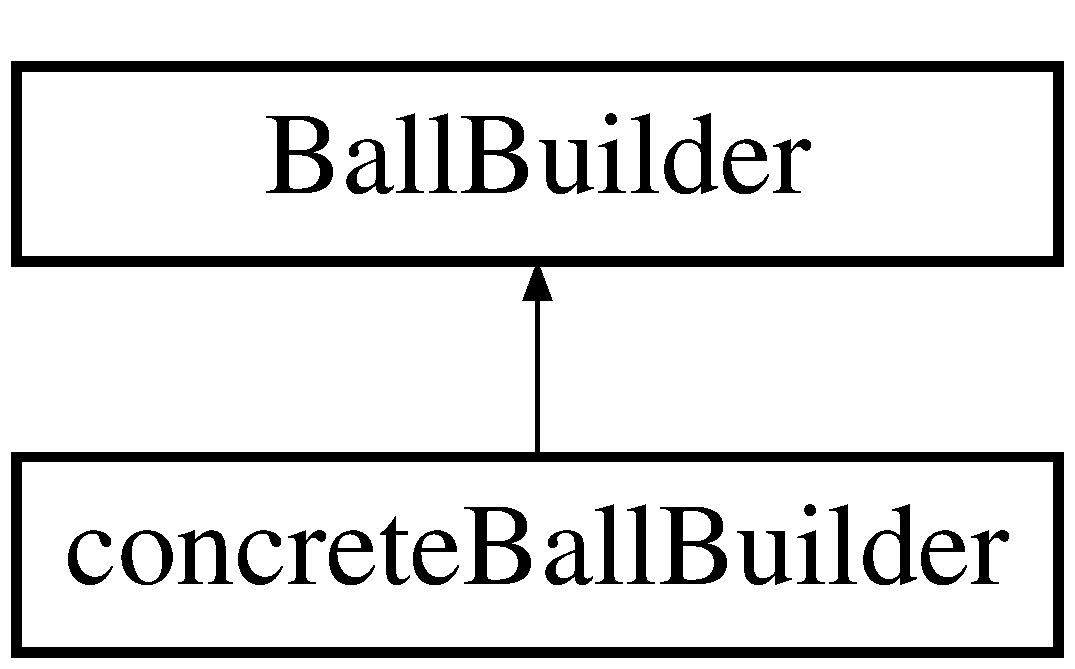
\includegraphics[height=2.000000cm]{class_ball_builder}
\end{center}
\end{figure}
\subsection*{Public Member Functions}
\begin{DoxyCompactItemize}
\item 
virtual void \mbox{\hyperlink{class_ball_builder_a5dc064067607fa4ef22db5901cca9e62}{build\+Ball}} ()
\item 
virtual void \mbox{\hyperlink{class_ball_builder_a0ca1344197192ea0f5aa5b7104e5f876}{build\+Coordinate}} (\mbox{\hyperlink{class_coordinate}{Coordinate}} c)
\item 
virtual void \mbox{\hyperlink{class_ball_builder_a0cd696c49074e3923a76ec8aed10ad45}{build\+Color}} (Q\+String color)
\item 
virtual void \mbox{\hyperlink{class_ball_builder_a6514a4ef81d56ba21708783cce473e4e}{build\+Mass}} (double mass)
\item 
virtual void \mbox{\hyperlink{class_ball_builder_af101d6eac3453fd0fda02b8900b49e8f}{build\+Radius}} (int radius)
\item 
virtual void \mbox{\hyperlink{class_ball_builder_a9139eedc191ad41fa221f06902646d4b}{build\+X\+Velocity}} (double xV)
\item 
virtual void \mbox{\hyperlink{class_ball_builder_a1687bc4c363f259dd38b0d7d6ac92e57}{build\+Y\+Velocity}} (double yV)
\end{DoxyCompactItemize}


\subsection{Detailed Description}
Ballbuilder class is the abstract builder class for object ball. 

\begin{DoxyAuthor}{Author}
Archibald Weng 
\end{DoxyAuthor}
\begin{DoxyDate}{Date}
April 2018 
\end{DoxyDate}


\subsection{Member Function Documentation}
\mbox{\Hypertarget{class_ball_builder_a5dc064067607fa4ef22db5901cca9e62}\label{class_ball_builder_a5dc064067607fa4ef22db5901cca9e62}} 
\index{Ball\+Builder@{Ball\+Builder}!build\+Ball@{build\+Ball}}
\index{build\+Ball@{build\+Ball}!Ball\+Builder@{Ball\+Builder}}
\subsubsection{\texorpdfstring{build\+Ball()}{buildBall()}}
{\footnotesize\ttfamily virtual void Ball\+Builder\+::build\+Ball (\begin{DoxyParamCaption}{ }\end{DoxyParamCaption})\hspace{0.3cm}{\ttfamily [inline]}, {\ttfamily [virtual]}}

build a ball 

Reimplemented in \mbox{\hyperlink{classconcrete_ball_builder_a882e6217ebab232ee2a3d0af63c43b5a}{concrete\+Ball\+Builder}}.

\mbox{\Hypertarget{class_ball_builder_a0cd696c49074e3923a76ec8aed10ad45}\label{class_ball_builder_a0cd696c49074e3923a76ec8aed10ad45}} 
\index{Ball\+Builder@{Ball\+Builder}!build\+Color@{build\+Color}}
\index{build\+Color@{build\+Color}!Ball\+Builder@{Ball\+Builder}}
\subsubsection{\texorpdfstring{build\+Color()}{buildColor()}}
{\footnotesize\ttfamily virtual void Ball\+Builder\+::build\+Color (\begin{DoxyParamCaption}\item[{Q\+String}]{color }\end{DoxyParamCaption})\hspace{0.3cm}{\ttfamily [inline]}, {\ttfamily [virtual]}}

set the ball\textquotesingle{}s color 

Reimplemented in \mbox{\hyperlink{classconcrete_ball_builder_afec6299653c5c810708254d3e32b6368}{concrete\+Ball\+Builder}}.

\mbox{\Hypertarget{class_ball_builder_a0ca1344197192ea0f5aa5b7104e5f876}\label{class_ball_builder_a0ca1344197192ea0f5aa5b7104e5f876}} 
\index{Ball\+Builder@{Ball\+Builder}!build\+Coordinate@{build\+Coordinate}}
\index{build\+Coordinate@{build\+Coordinate}!Ball\+Builder@{Ball\+Builder}}
\subsubsection{\texorpdfstring{build\+Coordinate()}{buildCoordinate()}}
{\footnotesize\ttfamily virtual void Ball\+Builder\+::build\+Coordinate (\begin{DoxyParamCaption}\item[{\mbox{\hyperlink{class_coordinate}{Coordinate}}}]{c }\end{DoxyParamCaption})\hspace{0.3cm}{\ttfamily [inline]}, {\ttfamily [virtual]}}

set the ball\textquotesingle{}s coordinate 

Reimplemented in \mbox{\hyperlink{classconcrete_ball_builder_ae4ddab3b62cc22f9f85d9bd3829830c4}{concrete\+Ball\+Builder}}.

\mbox{\Hypertarget{class_ball_builder_a6514a4ef81d56ba21708783cce473e4e}\label{class_ball_builder_a6514a4ef81d56ba21708783cce473e4e}} 
\index{Ball\+Builder@{Ball\+Builder}!build\+Mass@{build\+Mass}}
\index{build\+Mass@{build\+Mass}!Ball\+Builder@{Ball\+Builder}}
\subsubsection{\texorpdfstring{build\+Mass()}{buildMass()}}
{\footnotesize\ttfamily virtual void Ball\+Builder\+::build\+Mass (\begin{DoxyParamCaption}\item[{double}]{mass }\end{DoxyParamCaption})\hspace{0.3cm}{\ttfamily [inline]}, {\ttfamily [virtual]}}

set the ball\textquotesingle{}s mass 

Reimplemented in \mbox{\hyperlink{classconcrete_ball_builder_a74b84331ccf45c4880bf3a9bda6bfb22}{concrete\+Ball\+Builder}}.

\mbox{\Hypertarget{class_ball_builder_af101d6eac3453fd0fda02b8900b49e8f}\label{class_ball_builder_af101d6eac3453fd0fda02b8900b49e8f}} 
\index{Ball\+Builder@{Ball\+Builder}!build\+Radius@{build\+Radius}}
\index{build\+Radius@{build\+Radius}!Ball\+Builder@{Ball\+Builder}}
\subsubsection{\texorpdfstring{build\+Radius()}{buildRadius()}}
{\footnotesize\ttfamily virtual void Ball\+Builder\+::build\+Radius (\begin{DoxyParamCaption}\item[{int}]{radius }\end{DoxyParamCaption})\hspace{0.3cm}{\ttfamily [inline]}, {\ttfamily [virtual]}}

set the ball\textquotesingle{}s radius 

Reimplemented in \mbox{\hyperlink{classconcrete_ball_builder_aa85cf84c6c3cf21e9e4ad83c250d0e58}{concrete\+Ball\+Builder}}.

\mbox{\Hypertarget{class_ball_builder_a9139eedc191ad41fa221f06902646d4b}\label{class_ball_builder_a9139eedc191ad41fa221f06902646d4b}} 
\index{Ball\+Builder@{Ball\+Builder}!build\+X\+Velocity@{build\+X\+Velocity}}
\index{build\+X\+Velocity@{build\+X\+Velocity}!Ball\+Builder@{Ball\+Builder}}
\subsubsection{\texorpdfstring{build\+X\+Velocity()}{buildXVelocity()}}
{\footnotesize\ttfamily virtual void Ball\+Builder\+::build\+X\+Velocity (\begin{DoxyParamCaption}\item[{double}]{xV }\end{DoxyParamCaption})\hspace{0.3cm}{\ttfamily [inline]}, {\ttfamily [virtual]}}

set the ball\textquotesingle{}s x velocity 

Reimplemented in \mbox{\hyperlink{classconcrete_ball_builder_a45c8c4aaf54af6e5f619ccc3d0c62924}{concrete\+Ball\+Builder}}.

\mbox{\Hypertarget{class_ball_builder_a1687bc4c363f259dd38b0d7d6ac92e57}\label{class_ball_builder_a1687bc4c363f259dd38b0d7d6ac92e57}} 
\index{Ball\+Builder@{Ball\+Builder}!build\+Y\+Velocity@{build\+Y\+Velocity}}
\index{build\+Y\+Velocity@{build\+Y\+Velocity}!Ball\+Builder@{Ball\+Builder}}
\subsubsection{\texorpdfstring{build\+Y\+Velocity()}{buildYVelocity()}}
{\footnotesize\ttfamily virtual void Ball\+Builder\+::build\+Y\+Velocity (\begin{DoxyParamCaption}\item[{double}]{yV }\end{DoxyParamCaption})\hspace{0.3cm}{\ttfamily [inline]}, {\ttfamily [virtual]}}

set the ball\textquotesingle{}s y velocity 

Reimplemented in \mbox{\hyperlink{classconcrete_ball_builder_a6054b9012af3247b16f2e1c4040555cb}{concrete\+Ball\+Builder}}.



The documentation for this class was generated from the following files\+:\begin{DoxyCompactItemize}
\item 
ballbuilder.\+h\item 
ballbuilder.\+cpp\end{DoxyCompactItemize}

\hypertarget{classconcrete_ball_builder}{}\section{concrete\+Ball\+Builder Class Reference}
\label{classconcrete_ball_builder}\index{concrete\+Ball\+Builder@{concrete\+Ball\+Builder}}


Concrete\+Ball\+Builder class is the concrete builder class for object ball.  




{\ttfamily \#include $<$concreteballbuilder.\+h$>$}

Inheritance diagram for concrete\+Ball\+Builder\+:\begin{figure}[H]
\begin{center}
\leavevmode
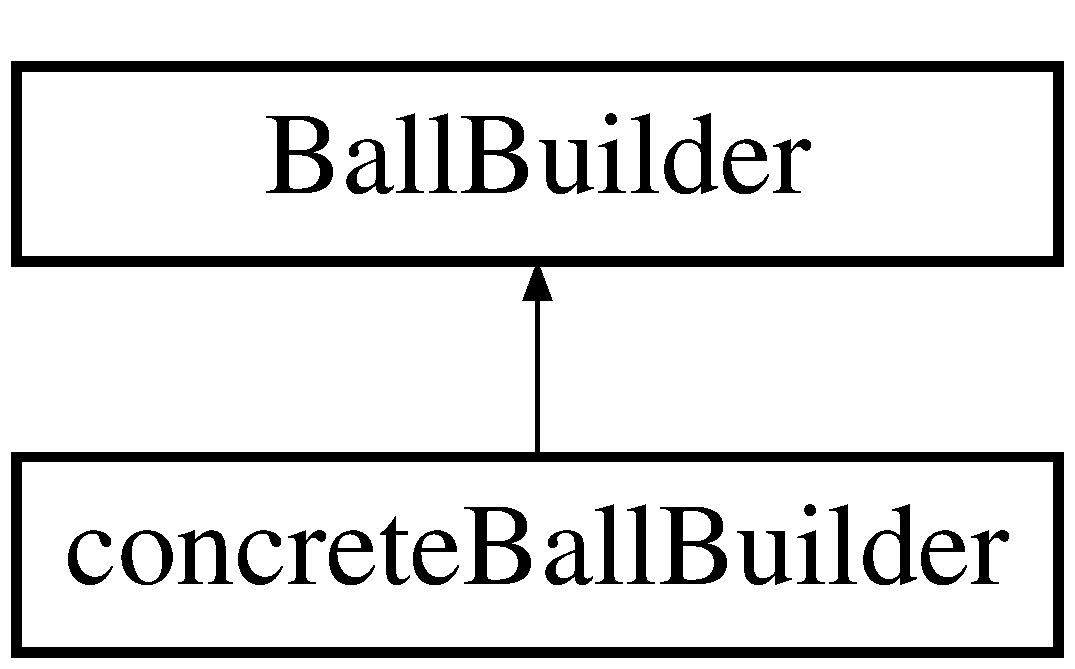
\includegraphics[height=2.000000cm]{classconcrete_ball_builder}
\end{center}
\end{figure}
\subsection*{Public Member Functions}
\begin{DoxyCompactItemize}
\item 
\mbox{\Hypertarget{classconcrete_ball_builder_a9085a8f83babb942502ebc105ce01b34}\label{classconcrete_ball_builder_a9085a8f83babb942502ebc105ce01b34}} 
{\bfseries concrete\+Ball\+Builder} (\mbox{\hyperlink{class_stage1_factory}{Stage1\+Factory}} $\ast$factory)
\item 
virtual void \mbox{\hyperlink{classconcrete_ball_builder_a882e6217ebab232ee2a3d0af63c43b5a}{build\+Ball}} ()
\item 
virtual void \mbox{\hyperlink{classconcrete_ball_builder_ae4ddab3b62cc22f9f85d9bd3829830c4}{build\+Coordinate}} (\mbox{\hyperlink{class_coordinate}{Coordinate}} c)
\item 
virtual void \mbox{\hyperlink{classconcrete_ball_builder_afec6299653c5c810708254d3e32b6368}{build\+Color}} (Q\+String color)
\item 
virtual void \mbox{\hyperlink{classconcrete_ball_builder_a74b84331ccf45c4880bf3a9bda6bfb22}{build\+Mass}} (double mass)
\item 
virtual void \mbox{\hyperlink{classconcrete_ball_builder_aa85cf84c6c3cf21e9e4ad83c250d0e58}{build\+Radius}} (int radius)
\item 
virtual void \mbox{\hyperlink{classconcrete_ball_builder_a45c8c4aaf54af6e5f619ccc3d0c62924}{build\+X\+Velocity}} (double xV)
\item 
virtual void \mbox{\hyperlink{classconcrete_ball_builder_a6054b9012af3247b16f2e1c4040555cb}{build\+Y\+Velocity}} (double yV)
\item 
virtual \mbox{\hyperlink{class_ball}{Ball}} $\ast$ \mbox{\hyperlink{classconcrete_ball_builder_a31311259bb9ba3580b4a0b190cbc938b}{get\+Ball}} ()
\end{DoxyCompactItemize}
\subsection*{Protected Attributes}
\begin{DoxyCompactItemize}
\item 
\mbox{\Hypertarget{classconcrete_ball_builder_aa2a91379bfc8d7ffcece63ff69ff7940}\label{classconcrete_ball_builder_aa2a91379bfc8d7ffcece63ff69ff7940}} 
\mbox{\hyperlink{class_ball}{Ball}} $\ast$ {\bfseries ball}
\item 
\mbox{\Hypertarget{classconcrete_ball_builder_a6d70af8ab25d8143a26d18cd65476290}\label{classconcrete_ball_builder_a6d70af8ab25d8143a26d18cd65476290}} 
\mbox{\hyperlink{class_game_factory}{Game\+Factory}} $\ast$ {\bfseries m\+\_\+factory}
\end{DoxyCompactItemize}


\subsection{Detailed Description}
Concrete\+Ball\+Builder class is the concrete builder class for object ball. 

\begin{DoxyAuthor}{Author}
Archibald Weng 
\end{DoxyAuthor}
\begin{DoxyDate}{Date}
April 2018 
\end{DoxyDate}


\subsection{Member Function Documentation}
\mbox{\Hypertarget{classconcrete_ball_builder_a882e6217ebab232ee2a3d0af63c43b5a}\label{classconcrete_ball_builder_a882e6217ebab232ee2a3d0af63c43b5a}} 
\index{concrete\+Ball\+Builder@{concrete\+Ball\+Builder}!build\+Ball@{build\+Ball}}
\index{build\+Ball@{build\+Ball}!concrete\+Ball\+Builder@{concrete\+Ball\+Builder}}
\subsubsection{\texorpdfstring{build\+Ball()}{buildBall()}}
{\footnotesize\ttfamily virtual void concrete\+Ball\+Builder\+::build\+Ball (\begin{DoxyParamCaption}{ }\end{DoxyParamCaption})\hspace{0.3cm}{\ttfamily [inline]}, {\ttfamily [virtual]}}

build a ball 

Reimplemented from \mbox{\hyperlink{class_ball_builder_a5dc064067607fa4ef22db5901cca9e62}{Ball\+Builder}}.

\mbox{\Hypertarget{classconcrete_ball_builder_afec6299653c5c810708254d3e32b6368}\label{classconcrete_ball_builder_afec6299653c5c810708254d3e32b6368}} 
\index{concrete\+Ball\+Builder@{concrete\+Ball\+Builder}!build\+Color@{build\+Color}}
\index{build\+Color@{build\+Color}!concrete\+Ball\+Builder@{concrete\+Ball\+Builder}}
\subsubsection{\texorpdfstring{build\+Color()}{buildColor()}}
{\footnotesize\ttfamily virtual void concrete\+Ball\+Builder\+::build\+Color (\begin{DoxyParamCaption}\item[{Q\+String}]{color }\end{DoxyParamCaption})\hspace{0.3cm}{\ttfamily [inline]}, {\ttfamily [virtual]}}

set the ball\textquotesingle{}s color 

Reimplemented from \mbox{\hyperlink{class_ball_builder_a0cd696c49074e3923a76ec8aed10ad45}{Ball\+Builder}}.

\mbox{\Hypertarget{classconcrete_ball_builder_ae4ddab3b62cc22f9f85d9bd3829830c4}\label{classconcrete_ball_builder_ae4ddab3b62cc22f9f85d9bd3829830c4}} 
\index{concrete\+Ball\+Builder@{concrete\+Ball\+Builder}!build\+Coordinate@{build\+Coordinate}}
\index{build\+Coordinate@{build\+Coordinate}!concrete\+Ball\+Builder@{concrete\+Ball\+Builder}}
\subsubsection{\texorpdfstring{build\+Coordinate()}{buildCoordinate()}}
{\footnotesize\ttfamily virtual void concrete\+Ball\+Builder\+::build\+Coordinate (\begin{DoxyParamCaption}\item[{\mbox{\hyperlink{class_coordinate}{Coordinate}}}]{c }\end{DoxyParamCaption})\hspace{0.3cm}{\ttfamily [inline]}, {\ttfamily [virtual]}}

set the ball\textquotesingle{}s coordinate 

Reimplemented from \mbox{\hyperlink{class_ball_builder_a0ca1344197192ea0f5aa5b7104e5f876}{Ball\+Builder}}.

\mbox{\Hypertarget{classconcrete_ball_builder_a74b84331ccf45c4880bf3a9bda6bfb22}\label{classconcrete_ball_builder_a74b84331ccf45c4880bf3a9bda6bfb22}} 
\index{concrete\+Ball\+Builder@{concrete\+Ball\+Builder}!build\+Mass@{build\+Mass}}
\index{build\+Mass@{build\+Mass}!concrete\+Ball\+Builder@{concrete\+Ball\+Builder}}
\subsubsection{\texorpdfstring{build\+Mass()}{buildMass()}}
{\footnotesize\ttfamily virtual void concrete\+Ball\+Builder\+::build\+Mass (\begin{DoxyParamCaption}\item[{double}]{mass }\end{DoxyParamCaption})\hspace{0.3cm}{\ttfamily [inline]}, {\ttfamily [virtual]}}

set the ball\textquotesingle{}s mass 

Reimplemented from \mbox{\hyperlink{class_ball_builder_a6514a4ef81d56ba21708783cce473e4e}{Ball\+Builder}}.

\mbox{\Hypertarget{classconcrete_ball_builder_aa85cf84c6c3cf21e9e4ad83c250d0e58}\label{classconcrete_ball_builder_aa85cf84c6c3cf21e9e4ad83c250d0e58}} 
\index{concrete\+Ball\+Builder@{concrete\+Ball\+Builder}!build\+Radius@{build\+Radius}}
\index{build\+Radius@{build\+Radius}!concrete\+Ball\+Builder@{concrete\+Ball\+Builder}}
\subsubsection{\texorpdfstring{build\+Radius()}{buildRadius()}}
{\footnotesize\ttfamily virtual void concrete\+Ball\+Builder\+::build\+Radius (\begin{DoxyParamCaption}\item[{int}]{radius }\end{DoxyParamCaption})\hspace{0.3cm}{\ttfamily [inline]}, {\ttfamily [virtual]}}

set the ball\textquotesingle{}s radius 

Reimplemented from \mbox{\hyperlink{class_ball_builder_af101d6eac3453fd0fda02b8900b49e8f}{Ball\+Builder}}.

\mbox{\Hypertarget{classconcrete_ball_builder_a45c8c4aaf54af6e5f619ccc3d0c62924}\label{classconcrete_ball_builder_a45c8c4aaf54af6e5f619ccc3d0c62924}} 
\index{concrete\+Ball\+Builder@{concrete\+Ball\+Builder}!build\+X\+Velocity@{build\+X\+Velocity}}
\index{build\+X\+Velocity@{build\+X\+Velocity}!concrete\+Ball\+Builder@{concrete\+Ball\+Builder}}
\subsubsection{\texorpdfstring{build\+X\+Velocity()}{buildXVelocity()}}
{\footnotesize\ttfamily virtual void concrete\+Ball\+Builder\+::build\+X\+Velocity (\begin{DoxyParamCaption}\item[{double}]{xV }\end{DoxyParamCaption})\hspace{0.3cm}{\ttfamily [inline]}, {\ttfamily [virtual]}}

set the ball\textquotesingle{}s x velocity 

Reimplemented from \mbox{\hyperlink{class_ball_builder_a9139eedc191ad41fa221f06902646d4b}{Ball\+Builder}}.

\mbox{\Hypertarget{classconcrete_ball_builder_a6054b9012af3247b16f2e1c4040555cb}\label{classconcrete_ball_builder_a6054b9012af3247b16f2e1c4040555cb}} 
\index{concrete\+Ball\+Builder@{concrete\+Ball\+Builder}!build\+Y\+Velocity@{build\+Y\+Velocity}}
\index{build\+Y\+Velocity@{build\+Y\+Velocity}!concrete\+Ball\+Builder@{concrete\+Ball\+Builder}}
\subsubsection{\texorpdfstring{build\+Y\+Velocity()}{buildYVelocity()}}
{\footnotesize\ttfamily virtual void concrete\+Ball\+Builder\+::build\+Y\+Velocity (\begin{DoxyParamCaption}\item[{double}]{yV }\end{DoxyParamCaption})\hspace{0.3cm}{\ttfamily [inline]}, {\ttfamily [virtual]}}

set the ball\textquotesingle{}s y velocity 

Reimplemented from \mbox{\hyperlink{class_ball_builder_a1687bc4c363f259dd38b0d7d6ac92e57}{Ball\+Builder}}.

\mbox{\Hypertarget{classconcrete_ball_builder_a31311259bb9ba3580b4a0b190cbc938b}\label{classconcrete_ball_builder_a31311259bb9ba3580b4a0b190cbc938b}} 
\index{concrete\+Ball\+Builder@{concrete\+Ball\+Builder}!get\+Ball@{get\+Ball}}
\index{get\+Ball@{get\+Ball}!concrete\+Ball\+Builder@{concrete\+Ball\+Builder}}
\subsubsection{\texorpdfstring{get\+Ball()}{getBall()}}
{\footnotesize\ttfamily virtual \mbox{\hyperlink{class_ball}{Ball}}$\ast$ concrete\+Ball\+Builder\+::get\+Ball (\begin{DoxyParamCaption}{ }\end{DoxyParamCaption})\hspace{0.3cm}{\ttfamily [inline]}, {\ttfamily [virtual]}}

return the ball built by this builder 

The documentation for this class was generated from the following file\+:\begin{DoxyCompactItemize}
\item 
concreteballbuilder.\+h\end{DoxyCompactItemize}

\hypertarget{class_concrete_table_builder}{}\section{Concrete\+Table\+Builder Class Reference}
\label{class_concrete_table_builder}\index{Concrete\+Table\+Builder@{Concrete\+Table\+Builder}}


\mbox{\hyperlink{class_concrete_table_builder}{Concrete\+Table\+Builder}} class is the concrete builder class for object table.  




{\ttfamily \#include $<$concretetablebuilder.\+h$>$}

Inheritance diagram for Concrete\+Table\+Builder\+:\begin{figure}[H]
\begin{center}
\leavevmode
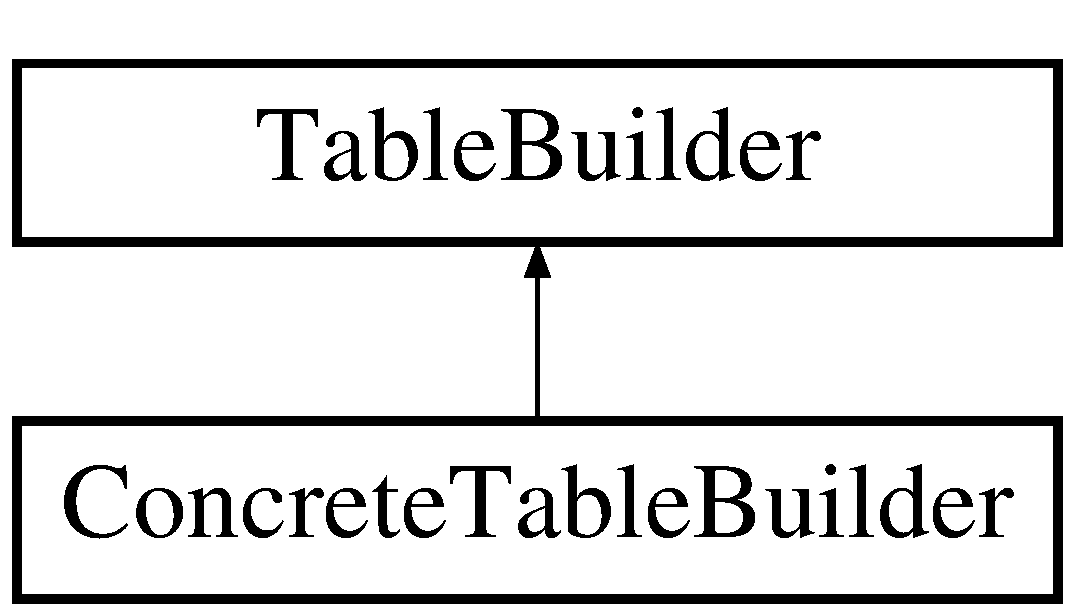
\includegraphics[height=2.000000cm]{class_concrete_table_builder}
\end{center}
\end{figure}
\subsection*{Public Member Functions}
\begin{DoxyCompactItemize}
\item 
\mbox{\hyperlink{class_concrete_table_builder_aff8b7c167d68b9e71c18888136b53034}{Concrete\+Table\+Builder}} (\mbox{\hyperlink{class_stage1_factory}{Stage1\+Factory}} $\ast$facotry)
\item 
virtual void \mbox{\hyperlink{class_concrete_table_builder_af49b5e371e6f725303e4b2f011d20fad}{build\+Table}} ()
\item 
virtual void \mbox{\hyperlink{class_concrete_table_builder_a154545f9b286b6a9ccff09a28c7a644d}{build\+Width}} (int width)
\item 
virtual void \mbox{\hyperlink{class_concrete_table_builder_a3e72d6d46e47146e385fff3937718a13}{build\+Height}} (int height)
\item 
virtual void \mbox{\hyperlink{class_concrete_table_builder_a547c26af597d109dbaf9b4de32f041a9}{build\+Background\+Color}} (Q\+String color)
\item 
virtual void \mbox{\hyperlink{class_concrete_table_builder_aab2c2ff234def292f7ead072dd5fda60}{build\+Friction}} (double friction)
\item 
virtual \mbox{\hyperlink{class_table}{Table}} $\ast$ \mbox{\hyperlink{class_concrete_table_builder_a0c1d21df18d11686736b84929deb669e}{get\+Table}} ()
\end{DoxyCompactItemize}
\subsection*{Protected Attributes}
\begin{DoxyCompactItemize}
\item 
\mbox{\Hypertarget{class_concrete_table_builder_ac04fa93314b700665c56fea05b9a0ff0}\label{class_concrete_table_builder_ac04fa93314b700665c56fea05b9a0ff0}} 
\mbox{\hyperlink{class_game_factory}{Game\+Factory}} $\ast$ {\bfseries m\+\_\+factory}
\item 
\mbox{\Hypertarget{class_concrete_table_builder_a1600f15904dd5029470bd93f0ccd206f}\label{class_concrete_table_builder_a1600f15904dd5029470bd93f0ccd206f}} 
\mbox{\hyperlink{class_table}{Table}} $\ast$ {\bfseries m\+\_\+table}
\end{DoxyCompactItemize}


\subsection{Detailed Description}
\mbox{\hyperlink{class_concrete_table_builder}{Concrete\+Table\+Builder}} class is the concrete builder class for object table. 

\begin{DoxyAuthor}{Author}
Archibald Weng 
\end{DoxyAuthor}
\begin{DoxyDate}{Date}
April 2018 
\end{DoxyDate}


\subsection{Constructor \& Destructor Documentation}
\mbox{\Hypertarget{class_concrete_table_builder_aff8b7c167d68b9e71c18888136b53034}\label{class_concrete_table_builder_aff8b7c167d68b9e71c18888136b53034}} 
\index{Concrete\+Table\+Builder@{Concrete\+Table\+Builder}!Concrete\+Table\+Builder@{Concrete\+Table\+Builder}}
\index{Concrete\+Table\+Builder@{Concrete\+Table\+Builder}!Concrete\+Table\+Builder@{Concrete\+Table\+Builder}}
\subsubsection{\texorpdfstring{Concrete\+Table\+Builder()}{ConcreteTableBuilder()}}
{\footnotesize\ttfamily Concrete\+Table\+Builder\+::\+Concrete\+Table\+Builder (\begin{DoxyParamCaption}\item[{\mbox{\hyperlink{class_stage1_factory}{Stage1\+Factory}} $\ast$}]{facotry }\end{DoxyParamCaption})\hspace{0.3cm}{\ttfamily [inline]}}

set the factory 

\subsection{Member Function Documentation}
\mbox{\Hypertarget{class_concrete_table_builder_a547c26af597d109dbaf9b4de32f041a9}\label{class_concrete_table_builder_a547c26af597d109dbaf9b4de32f041a9}} 
\index{Concrete\+Table\+Builder@{Concrete\+Table\+Builder}!build\+Background\+Color@{build\+Background\+Color}}
\index{build\+Background\+Color@{build\+Background\+Color}!Concrete\+Table\+Builder@{Concrete\+Table\+Builder}}
\subsubsection{\texorpdfstring{build\+Background\+Color()}{buildBackgroundColor()}}
{\footnotesize\ttfamily virtual void Concrete\+Table\+Builder\+::build\+Background\+Color (\begin{DoxyParamCaption}\item[{Q\+String}]{color }\end{DoxyParamCaption})\hspace{0.3cm}{\ttfamily [inline]}, {\ttfamily [virtual]}}

set the table\textquotesingle{}scolor 

Reimplemented from \mbox{\hyperlink{class_table_builder_a43bfcc7fbc5c45c0e2fe579b7d7e5f9c}{Table\+Builder}}.

\mbox{\Hypertarget{class_concrete_table_builder_aab2c2ff234def292f7ead072dd5fda60}\label{class_concrete_table_builder_aab2c2ff234def292f7ead072dd5fda60}} 
\index{Concrete\+Table\+Builder@{Concrete\+Table\+Builder}!build\+Friction@{build\+Friction}}
\index{build\+Friction@{build\+Friction}!Concrete\+Table\+Builder@{Concrete\+Table\+Builder}}
\subsubsection{\texorpdfstring{build\+Friction()}{buildFriction()}}
{\footnotesize\ttfamily virtual void Concrete\+Table\+Builder\+::build\+Friction (\begin{DoxyParamCaption}\item[{double}]{friction }\end{DoxyParamCaption})\hspace{0.3cm}{\ttfamily [inline]}, {\ttfamily [virtual]}}

set the table\textquotesingle{}s friction 

Reimplemented from \mbox{\hyperlink{class_table_builder_a02a8d4ae71a3ef43ffd283ac10aa2e19}{Table\+Builder}}.

\mbox{\Hypertarget{class_concrete_table_builder_a3e72d6d46e47146e385fff3937718a13}\label{class_concrete_table_builder_a3e72d6d46e47146e385fff3937718a13}} 
\index{Concrete\+Table\+Builder@{Concrete\+Table\+Builder}!build\+Height@{build\+Height}}
\index{build\+Height@{build\+Height}!Concrete\+Table\+Builder@{Concrete\+Table\+Builder}}
\subsubsection{\texorpdfstring{build\+Height()}{buildHeight()}}
{\footnotesize\ttfamily virtual void Concrete\+Table\+Builder\+::build\+Height (\begin{DoxyParamCaption}\item[{int}]{height }\end{DoxyParamCaption})\hspace{0.3cm}{\ttfamily [inline]}, {\ttfamily [virtual]}}

set the table\textquotesingle{}s height 

Reimplemented from \mbox{\hyperlink{class_table_builder_ad3e3bb11cd8f9eecd49ad6012e358d05}{Table\+Builder}}.

\mbox{\Hypertarget{class_concrete_table_builder_af49b5e371e6f725303e4b2f011d20fad}\label{class_concrete_table_builder_af49b5e371e6f725303e4b2f011d20fad}} 
\index{Concrete\+Table\+Builder@{Concrete\+Table\+Builder}!build\+Table@{build\+Table}}
\index{build\+Table@{build\+Table}!Concrete\+Table\+Builder@{Concrete\+Table\+Builder}}
\subsubsection{\texorpdfstring{build\+Table()}{buildTable()}}
{\footnotesize\ttfamily virtual void Concrete\+Table\+Builder\+::build\+Table (\begin{DoxyParamCaption}{ }\end{DoxyParamCaption})\hspace{0.3cm}{\ttfamily [inline]}, {\ttfamily [virtual]}}

build a table from the facotry 

Reimplemented from \mbox{\hyperlink{class_table_builder_a4aba0952fb1912f9ff7ca4cfb3085dd9}{Table\+Builder}}.

\mbox{\Hypertarget{class_concrete_table_builder_a154545f9b286b6a9ccff09a28c7a644d}\label{class_concrete_table_builder_a154545f9b286b6a9ccff09a28c7a644d}} 
\index{Concrete\+Table\+Builder@{Concrete\+Table\+Builder}!build\+Width@{build\+Width}}
\index{build\+Width@{build\+Width}!Concrete\+Table\+Builder@{Concrete\+Table\+Builder}}
\subsubsection{\texorpdfstring{build\+Width()}{buildWidth()}}
{\footnotesize\ttfamily virtual void Concrete\+Table\+Builder\+::build\+Width (\begin{DoxyParamCaption}\item[{int}]{width }\end{DoxyParamCaption})\hspace{0.3cm}{\ttfamily [inline]}, {\ttfamily [virtual]}}

set the table\textquotesingle{}s width \mbox{\Hypertarget{class_concrete_table_builder_a0c1d21df18d11686736b84929deb669e}\label{class_concrete_table_builder_a0c1d21df18d11686736b84929deb669e}} 
\index{Concrete\+Table\+Builder@{Concrete\+Table\+Builder}!get\+Table@{get\+Table}}
\index{get\+Table@{get\+Table}!Concrete\+Table\+Builder@{Concrete\+Table\+Builder}}
\subsubsection{\texorpdfstring{get\+Table()}{getTable()}}
{\footnotesize\ttfamily virtual \mbox{\hyperlink{class_table}{Table}}$\ast$ Concrete\+Table\+Builder\+::get\+Table (\begin{DoxyParamCaption}{ }\end{DoxyParamCaption})\hspace{0.3cm}{\ttfamily [inline]}, {\ttfamily [virtual]}}

get this table\textquotesingle{}s pointer 

The documentation for this class was generated from the following file\+:\begin{DoxyCompactItemize}
\item 
concretetablebuilder.\+h\end{DoxyCompactItemize}

\hypertarget{class_coordinate}{}\section{Coordinate Class Reference}
\label{class_coordinate}\index{Coordinate@{Coordinate}}


\mbox{\hyperlink{class_coordinate}{Coordinate}} class is for ball class to have a convienent way to store its position info.  




{\ttfamily \#include $<$coordinate.\+h$>$}

\subsection*{Public Member Functions}
\begin{DoxyCompactItemize}
\item 
\mbox{\Hypertarget{class_coordinate_a2abcffb39c9db2c4c69bc5d240d1105f}\label{class_coordinate_a2abcffb39c9db2c4c69bc5d240d1105f}} 
{\bfseries Coordinate} (unsigned int x\+Coordinate, unsigned int y\+Coordinate, unsigned int frame\+Width, unsigned int frame\+Height)
\item 
int \mbox{\hyperlink{class_coordinate_adb2d33e506b944b74cb45657152a6948}{get\+Qt\+Rendering\+X\+Coordinate}} ()
\item 
int \mbox{\hyperlink{class_coordinate_a3f71047bac34b137a58a6dcc5ab69df4}{get\+Qt\+Rendering\+Y\+Coordinate}} ()
\item 
void \mbox{\hyperlink{class_coordinate_a8481ba6f79f9b7f6ac41a28119d251b9}{change\+In\+X\+Coordinate}} (int change)
\item 
void \mbox{\hyperlink{class_coordinate_ad2cd26113f8101771bea445fb5dc907f}{change\+In\+Y\+Coordinate}} (int change)
\item 
void \mbox{\hyperlink{class_coordinate_a1ab7964582737b9bd19788e08a8a8c6b}{set\+Y\+Coordinate\+To\+Zero}} (int offset)
\item 
\mbox{\Hypertarget{class_coordinate_a1acb338ca5f143627f876e4dd6b8c93a}\label{class_coordinate_a1acb338ca5f143627f876e4dd6b8c93a}} 
unsigned int {\bfseries get\+X\+Coordinate} ()
\item 
\mbox{\Hypertarget{class_coordinate_ab7adec413c90e64f87592d9dd563f0c9}\label{class_coordinate_ab7adec413c90e64f87592d9dd563f0c9}} 
unsigned int {\bfseries get\+Y\+Coordinate} ()
\item 
\mbox{\Hypertarget{class_coordinate_ad39f3c1849a18c340c254d5e71093f98}\label{class_coordinate_ad39f3c1849a18c340c254d5e71093f98}} 
unsigned int {\bfseries get\+Frame\+Height} ()
\item 
\mbox{\Hypertarget{class_coordinate_a84058b1cc290474a88411afb16986444}\label{class_coordinate_a84058b1cc290474a88411afb16986444}} 
unsigned int {\bfseries get\+Frame\+Width} ()
\item 
\mbox{\Hypertarget{class_coordinate_a91fed770c781d4aaa493d3f44128e667}\label{class_coordinate_a91fed770c781d4aaa493d3f44128e667}} 
void {\bfseries set\+X\+Coordinate} (unsigned int x)
\item 
\mbox{\Hypertarget{class_coordinate_aea0d21e00aab864c4f0a2bbd6569a86e}\label{class_coordinate_aea0d21e00aab864c4f0a2bbd6569a86e}} 
void {\bfseries set\+Y\+Coordinate} (unsigned int y)
\end{DoxyCompactItemize}


\subsection{Detailed Description}
\mbox{\hyperlink{class_coordinate}{Coordinate}} class is for ball class to have a convienent way to store its position info. 

\begin{DoxyAuthor}{Author}
Archibald Weng 
\end{DoxyAuthor}
\begin{DoxyDate}{Date}
April 2018 
\end{DoxyDate}


\subsection{Member Function Documentation}
\mbox{\Hypertarget{class_coordinate_a8481ba6f79f9b7f6ac41a28119d251b9}\label{class_coordinate_a8481ba6f79f9b7f6ac41a28119d251b9}} 
\index{Coordinate@{Coordinate}!change\+In\+X\+Coordinate@{change\+In\+X\+Coordinate}}
\index{change\+In\+X\+Coordinate@{change\+In\+X\+Coordinate}!Coordinate@{Coordinate}}
\subsubsection{\texorpdfstring{change\+In\+X\+Coordinate()}{changeInXCoordinate()}}
{\footnotesize\ttfamily void Coordinate\+::change\+In\+X\+Coordinate (\begin{DoxyParamCaption}\item[{int}]{change }\end{DoxyParamCaption})}

change the X coordinate with \textquotesingle{}change\textquotesingle{} parameter \mbox{\Hypertarget{class_coordinate_ad2cd26113f8101771bea445fb5dc907f}\label{class_coordinate_ad2cd26113f8101771bea445fb5dc907f}} 
\index{Coordinate@{Coordinate}!change\+In\+Y\+Coordinate@{change\+In\+Y\+Coordinate}}
\index{change\+In\+Y\+Coordinate@{change\+In\+Y\+Coordinate}!Coordinate@{Coordinate}}
\subsubsection{\texorpdfstring{change\+In\+Y\+Coordinate()}{changeInYCoordinate()}}
{\footnotesize\ttfamily void Coordinate\+::change\+In\+Y\+Coordinate (\begin{DoxyParamCaption}\item[{int}]{change }\end{DoxyParamCaption})}

change the Y coordinate with \textquotesingle{}change\textquotesingle{} parameter \mbox{\Hypertarget{class_coordinate_adb2d33e506b944b74cb45657152a6948}\label{class_coordinate_adb2d33e506b944b74cb45657152a6948}} 
\index{Coordinate@{Coordinate}!get\+Qt\+Rendering\+X\+Coordinate@{get\+Qt\+Rendering\+X\+Coordinate}}
\index{get\+Qt\+Rendering\+X\+Coordinate@{get\+Qt\+Rendering\+X\+Coordinate}!Coordinate@{Coordinate}}
\subsubsection{\texorpdfstring{get\+Qt\+Rendering\+X\+Coordinate()}{getQtRenderingXCoordinate()}}
{\footnotesize\ttfamily int Coordinate\+::get\+Qt\+Rendering\+X\+Coordinate (\begin{DoxyParamCaption}{ }\end{DoxyParamCaption})}

return the X coordinate in Qt rendering version \mbox{\Hypertarget{class_coordinate_a3f71047bac34b137a58a6dcc5ab69df4}\label{class_coordinate_a3f71047bac34b137a58a6dcc5ab69df4}} 
\index{Coordinate@{Coordinate}!get\+Qt\+Rendering\+Y\+Coordinate@{get\+Qt\+Rendering\+Y\+Coordinate}}
\index{get\+Qt\+Rendering\+Y\+Coordinate@{get\+Qt\+Rendering\+Y\+Coordinate}!Coordinate@{Coordinate}}
\subsubsection{\texorpdfstring{get\+Qt\+Rendering\+Y\+Coordinate()}{getQtRenderingYCoordinate()}}
{\footnotesize\ttfamily int Coordinate\+::get\+Qt\+Rendering\+Y\+Coordinate (\begin{DoxyParamCaption}{ }\end{DoxyParamCaption})}

return the Y coordinate in Qt rendering version \mbox{\Hypertarget{class_coordinate_a1ab7964582737b9bd19788e08a8a8c6b}\label{class_coordinate_a1ab7964582737b9bd19788e08a8a8c6b}} 
\index{Coordinate@{Coordinate}!set\+Y\+Coordinate\+To\+Zero@{set\+Y\+Coordinate\+To\+Zero}}
\index{set\+Y\+Coordinate\+To\+Zero@{set\+Y\+Coordinate\+To\+Zero}!Coordinate@{Coordinate}}
\subsubsection{\texorpdfstring{set\+Y\+Coordinate\+To\+Zero()}{setYCoordinateToZero()}}
{\footnotesize\ttfamily void Coordinate\+::set\+Y\+Coordinate\+To\+Zero (\begin{DoxyParamCaption}\item[{int}]{offset }\end{DoxyParamCaption})}

set Y coordinate to zere 

The documentation for this class was generated from the following files\+:\begin{DoxyCompactItemize}
\item 
coordinate.\+h\item 
coordinate.\+cpp\end{DoxyCompactItemize}

\hypertarget{class_dialog}{}\section{Dialog Class Reference}
\label{class_dialog}\index{Dialog@{Dialog}}
Inheritance diagram for Dialog\+:\begin{figure}[H]
\begin{center}
\leavevmode
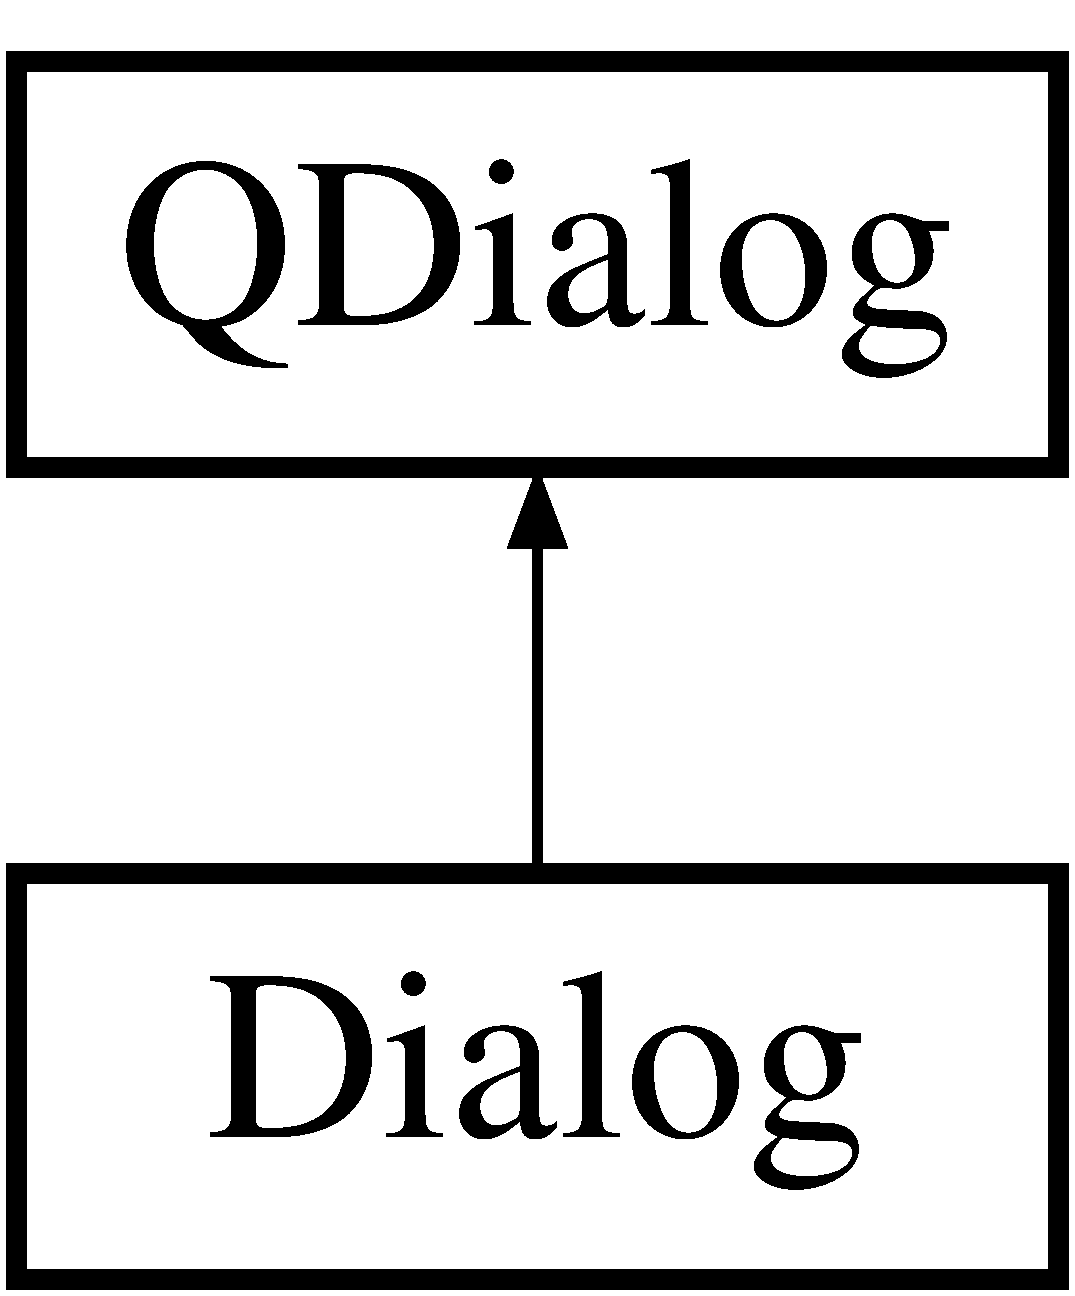
\includegraphics[height=2.000000cm]{class_dialog}
\end{center}
\end{figure}
\subsection*{Public Slots}
\begin{DoxyCompactItemize}
\item 
\mbox{\Hypertarget{class_dialog_a8bc4fe3b0cc12033369b49eab8751e14}\label{class_dialog_a8bc4fe3b0cc12033369b49eab8751e14}} 
void {\bfseries next\+Frame} ()
\item 
\mbox{\Hypertarget{class_dialog_a7760d4357317544538ea9815af13c4c7}\label{class_dialog_a7760d4357317544538ea9815af13c4c7}} 
void {\bfseries set\+Balls} (std\+::vector$<$ \mbox{\hyperlink{class_ball}{Ball}} $\ast$$>$ balls)
\end{DoxyCompactItemize}
\subsection*{Public Member Functions}
\begin{DoxyCompactItemize}
\item 
\mbox{\Hypertarget{class_dialog_acfa2063f9f962d394c6a645b6e7e08d8}\label{class_dialog_acfa2063f9f962d394c6a645b6e7e08d8}} 
{\bfseries Dialog} (Q\+Widget $\ast$parent=0)
\item 
void \mbox{\hyperlink{class_dialog_a4be1977cc02114a71dd2d43e7e27b6ff}{add\+Ball}} (\mbox{\hyperlink{class_ball}{Ball}} $\ast$b)
\item 
void \mbox{\hyperlink{class_dialog_a072907acf851676f20f018ee27766ab9}{set\+Friction}} (double friction=0.\+1)
\end{DoxyCompactItemize}
\subsection*{Protected Member Functions}
\begin{DoxyCompactItemize}
\item 
\mbox{\Hypertarget{class_dialog_ac761f05fce616d76acf0612370b857ad}\label{class_dialog_ac761f05fce616d76acf0612370b857ad}} 
void {\bfseries paint\+Event} (Q\+Paint\+Event $\ast$event)
\end{DoxyCompactItemize}


\subsection{Member Function Documentation}
\mbox{\Hypertarget{class_dialog_a4be1977cc02114a71dd2d43e7e27b6ff}\label{class_dialog_a4be1977cc02114a71dd2d43e7e27b6ff}} 
\index{Dialog@{Dialog}!add\+Ball@{add\+Ball}}
\index{add\+Ball@{add\+Ball}!Dialog@{Dialog}}
\subsubsection{\texorpdfstring{add\+Ball()}{addBall()}}
{\footnotesize\ttfamily void Dialog\+::add\+Ball (\begin{DoxyParamCaption}\item[{\mbox{\hyperlink{class_ball}{Ball}} $\ast$}]{b }\end{DoxyParamCaption})}

add one ball to the visualization tool \mbox{\hyperlink{class_dialog}{Dialog}} \mbox{\Hypertarget{class_dialog_a072907acf851676f20f018ee27766ab9}\label{class_dialog_a072907acf851676f20f018ee27766ab9}} 
\index{Dialog@{Dialog}!set\+Friction@{set\+Friction}}
\index{set\+Friction@{set\+Friction}!Dialog@{Dialog}}
\subsubsection{\texorpdfstring{set\+Friction()}{setFriction()}}
{\footnotesize\ttfamily void Dialog\+::set\+Friction (\begin{DoxyParamCaption}\item[{double}]{friction = {\ttfamily 0.1} }\end{DoxyParamCaption})\hspace{0.3cm}{\ttfamily [inline]}}

set the friction to \mbox{\hyperlink{class_dialog}{Dialog}} 

The documentation for this class was generated from the following files\+:\begin{DoxyCompactItemize}
\item 
dialog.\+h\item 
dialog.\+cpp\end{DoxyCompactItemize}

\hypertarget{class_game_factory}{}\section{Game\+Factory Class Reference}
\label{class_game_factory}\index{Game\+Factory@{Game\+Factory}}


This is the abstract factory class in abstract factory method.  




{\ttfamily \#include $<$gamefactory.\+h$>$}

Inheritance diagram for Game\+Factory\+:\begin{figure}[H]
\begin{center}
\leavevmode
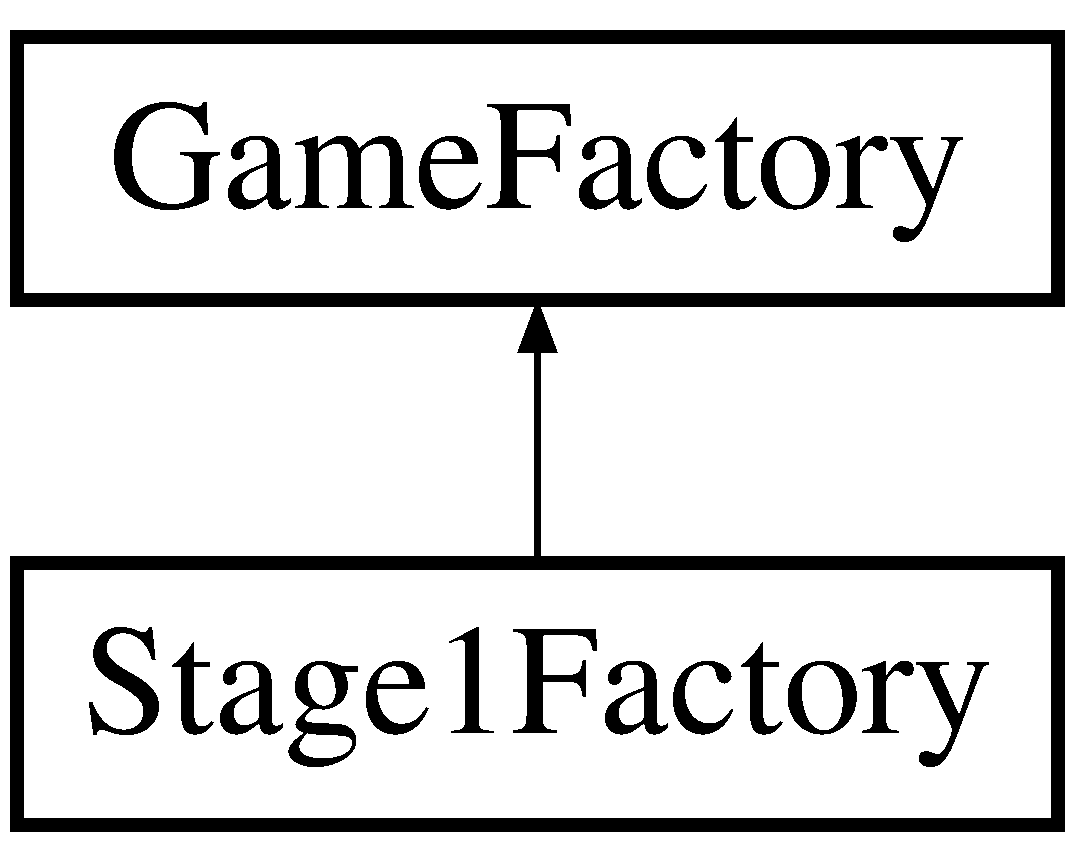
\includegraphics[height=2.000000cm]{class_game_factory}
\end{center}
\end{figure}
\subsection*{Public Member Functions}
\begin{DoxyCompactItemize}
\item 
virtual \mbox{\hyperlink{class_table}{Table}} $\ast$ \mbox{\hyperlink{class_game_factory_ac2e32aa1f1c55aae847745575afb0583}{create\+Table}} ()
\item 
virtual \mbox{\hyperlink{class_ball}{Ball}} $\ast$ \mbox{\hyperlink{class_game_factory_aae6fcb1b85abc73e3370246fdf77b7a8}{create\+Ball}} ()
\end{DoxyCompactItemize}


\subsection{Detailed Description}
This is the abstract factory class in abstract factory method. 

\begin{DoxyAuthor}{Author}
Archibald Weng 
\end{DoxyAuthor}
\begin{DoxyDate}{Date}
April 2018 
\end{DoxyDate}


\subsection{Member Function Documentation}
\mbox{\Hypertarget{class_game_factory_aae6fcb1b85abc73e3370246fdf77b7a8}\label{class_game_factory_aae6fcb1b85abc73e3370246fdf77b7a8}} 
\index{Game\+Factory@{Game\+Factory}!create\+Ball@{create\+Ball}}
\index{create\+Ball@{create\+Ball}!Game\+Factory@{Game\+Factory}}
\subsubsection{\texorpdfstring{create\+Ball()}{createBall()}}
{\footnotesize\ttfamily virtual \mbox{\hyperlink{class_ball}{Ball}}$\ast$ Game\+Factory\+::create\+Ball (\begin{DoxyParamCaption}{ }\end{DoxyParamCaption})\hspace{0.3cm}{\ttfamily [inline]}, {\ttfamily [virtual]}}

creation of the ball object 

Reimplemented in \mbox{\hyperlink{class_stage1_factory_a84b6d3dc3f6500cdc128bb553dacd4cc}{Stage1\+Factory}}.

\mbox{\Hypertarget{class_game_factory_ac2e32aa1f1c55aae847745575afb0583}\label{class_game_factory_ac2e32aa1f1c55aae847745575afb0583}} 
\index{Game\+Factory@{Game\+Factory}!create\+Table@{create\+Table}}
\index{create\+Table@{create\+Table}!Game\+Factory@{Game\+Factory}}
\subsubsection{\texorpdfstring{create\+Table()}{createTable()}}
{\footnotesize\ttfamily virtual \mbox{\hyperlink{class_table}{Table}}$\ast$ Game\+Factory\+::create\+Table (\begin{DoxyParamCaption}{ }\end{DoxyParamCaption})\hspace{0.3cm}{\ttfamily [inline]}, {\ttfamily [virtual]}}

creation of the table object 

Reimplemented in \mbox{\hyperlink{class_stage1_factory_ad1a070c87d52b00654125bd9f439cf26}{Stage1\+Factory}}.



The documentation for this class was generated from the following files\+:\begin{DoxyCompactItemize}
\item 
gamefactory.\+h\item 
gamefactory.\+cpp\end{DoxyCompactItemize}

\hypertarget{class_stage1_factory}{}\section{Stage1\+Factory Class Reference}
\label{class_stage1_factory}\index{Stage1\+Factory@{Stage1\+Factory}}


This is the concrete factory class in abstract factory method.  




{\ttfamily \#include $<$stage1factory.\+h$>$}

Inheritance diagram for Stage1\+Factory\+:\begin{figure}[H]
\begin{center}
\leavevmode
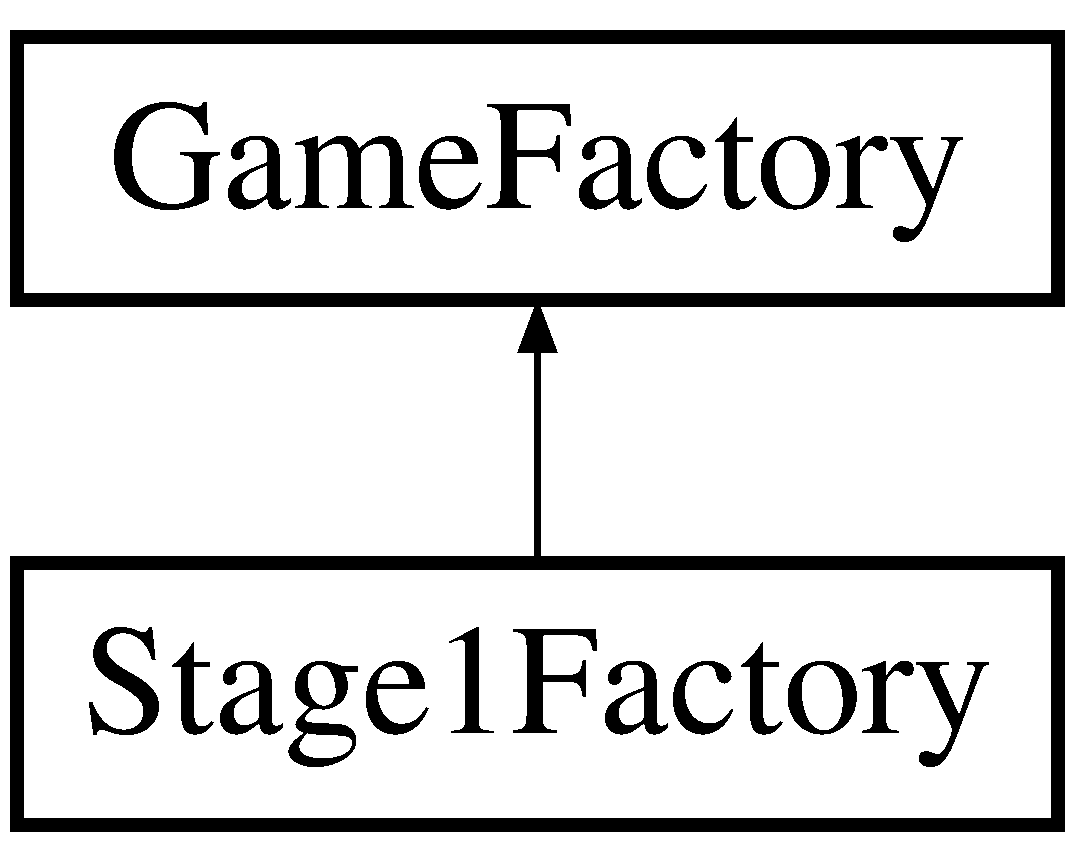
\includegraphics[height=2.000000cm]{class_stage1_factory}
\end{center}
\end{figure}
\subsection*{Public Member Functions}
\begin{DoxyCompactItemize}
\item 
\mbox{\hyperlink{class_table}{Table}} $\ast$ \mbox{\hyperlink{class_stage1_factory_ad1a070c87d52b00654125bd9f439cf26}{create\+Table}} ()
\item 
\mbox{\hyperlink{class_ball}{Ball}} $\ast$ \mbox{\hyperlink{class_stage1_factory_a84b6d3dc3f6500cdc128bb553dacd4cc}{create\+Ball}} ()
\end{DoxyCompactItemize}
\subsection*{Protected Attributes}
\begin{DoxyCompactItemize}
\item 
\mbox{\Hypertarget{class_stage1_factory_a82981d3a0cb0e98193e9176658d3e2ec}\label{class_stage1_factory_a82981d3a0cb0e98193e9176658d3e2ec}} 
\mbox{\hyperlink{class_table}{Table}} $\ast$ {\bfseries m\+\_\+table}
\item 
\mbox{\Hypertarget{class_stage1_factory_ad9cff77690b74d1e0cce4b24466bfff4}\label{class_stage1_factory_ad9cff77690b74d1e0cce4b24466bfff4}} 
\mbox{\hyperlink{class_ball}{Ball}} $\ast$ {\bfseries m\+\_\+ball}
\end{DoxyCompactItemize}


\subsection{Detailed Description}
This is the concrete factory class in abstract factory method. 

\begin{DoxyAuthor}{Author}
Archibald Weng 
\end{DoxyAuthor}
\begin{DoxyDate}{Date}
April 2018 
\end{DoxyDate}


\subsection{Member Function Documentation}
\mbox{\Hypertarget{class_stage1_factory_a84b6d3dc3f6500cdc128bb553dacd4cc}\label{class_stage1_factory_a84b6d3dc3f6500cdc128bb553dacd4cc}} 
\index{Stage1\+Factory@{Stage1\+Factory}!create\+Ball@{create\+Ball}}
\index{create\+Ball@{create\+Ball}!Stage1\+Factory@{Stage1\+Factory}}
\subsubsection{\texorpdfstring{create\+Ball()}{createBall()}}
{\footnotesize\ttfamily \mbox{\hyperlink{class_ball}{Ball}}$\ast$ Stage1\+Factory\+::create\+Ball (\begin{DoxyParamCaption}{ }\end{DoxyParamCaption})\hspace{0.3cm}{\ttfamily [inline]}, {\ttfamily [virtual]}}

creation of the ball object 

Reimplemented from \mbox{\hyperlink{class_game_factory_aae6fcb1b85abc73e3370246fdf77b7a8}{Game\+Factory}}.

\mbox{\Hypertarget{class_stage1_factory_ad1a070c87d52b00654125bd9f439cf26}\label{class_stage1_factory_ad1a070c87d52b00654125bd9f439cf26}} 
\index{Stage1\+Factory@{Stage1\+Factory}!create\+Table@{create\+Table}}
\index{create\+Table@{create\+Table}!Stage1\+Factory@{Stage1\+Factory}}
\subsubsection{\texorpdfstring{create\+Table()}{createTable()}}
{\footnotesize\ttfamily \mbox{\hyperlink{class_table}{Table}}$\ast$ Stage1\+Factory\+::create\+Table (\begin{DoxyParamCaption}{ }\end{DoxyParamCaption})\hspace{0.3cm}{\ttfamily [inline]}, {\ttfamily [virtual]}}

creation of the table object 

Reimplemented from \mbox{\hyperlink{class_game_factory_ac2e32aa1f1c55aae847745575afb0583}{Game\+Factory}}.



The documentation for this class was generated from the following files\+:\begin{DoxyCompactItemize}
\item 
stage1factory.\+h\item 
stage1factory.\+cpp\end{DoxyCompactItemize}

\hypertarget{class_table}{}\section{Table Class Reference}
\label{class_table}\index{Table@{Table}}


This is the class for table objects.  




{\ttfamily \#include $<$table.\+h$>$}

\subsection*{Public Member Functions}
\begin{DoxyCompactItemize}
\item 
\mbox{\Hypertarget{class_table_a3c30441a9209b449178cce0e0400c4f1}\label{class_table_a3c30441a9209b449178cce0e0400c4f1}} 
{\bfseries Table} (Q\+String color=\char`\"{}blue\char`\"{}, int width=300, int height=300, double friction=0.\+2)
\item 
\mbox{\Hypertarget{class_table_a5f633c6f4ba05cffe38333ef88374a8b}\label{class_table_a5f633c6f4ba05cffe38333ef88374a8b}} 
Q\+String {\bfseries get\+Color} ()
\item 
\mbox{\Hypertarget{class_table_af99d57a79ad07686c764f2fd7e016af8}\label{class_table_af99d57a79ad07686c764f2fd7e016af8}} 
int {\bfseries get\+Width} ()
\item 
\mbox{\Hypertarget{class_table_ac56d2b30a0bc0891cb43179fe12482f1}\label{class_table_ac56d2b30a0bc0891cb43179fe12482f1}} 
int {\bfseries get\+Height} ()
\item 
\mbox{\Hypertarget{class_table_a96e355deb9ff148fce509500df96ea6b}\label{class_table_a96e355deb9ff148fce509500df96ea6b}} 
double {\bfseries get\+Friction} ()
\item 
\mbox{\Hypertarget{class_table_aa21c02cdd032e5b8904f242e03af5f0e}\label{class_table_aa21c02cdd032e5b8904f242e03af5f0e}} 
void {\bfseries set\+Color} (Q\+String color)
\item 
\mbox{\Hypertarget{class_table_ab1f18aa925da6087701458104a09a0bc}\label{class_table_ab1f18aa925da6087701458104a09a0bc}} 
void {\bfseries set\+Width} (int width)
\item 
\mbox{\Hypertarget{class_table_add3f4e6e48b256ef70ca95b914185bd9}\label{class_table_add3f4e6e48b256ef70ca95b914185bd9}} 
void {\bfseries set\+Height} (int height)
\item 
\mbox{\Hypertarget{class_table_a2f6badebd4e196c6322954c393b5e39d}\label{class_table_a2f6badebd4e196c6322954c393b5e39d}} 
void {\bfseries set\+Friction} (double friction)
\end{DoxyCompactItemize}


\subsection{Detailed Description}
This is the class for table objects. 

\begin{DoxyAuthor}{Author}
Archibald Weng 
\end{DoxyAuthor}
\begin{DoxyDate}{Date}
April 2018 
\end{DoxyDate}


The documentation for this class was generated from the following file\+:\begin{DoxyCompactItemize}
\item 
table.\+h\end{DoxyCompactItemize}

\hypertarget{class_table_builder}{}\section{Table\+Builder Class Reference}
\label{class_table_builder}\index{Table\+Builder@{Table\+Builder}}


Tablebuilder class is the abstract builder class for object table.  




{\ttfamily \#include $<$tablebuilder.\+h$>$}

Inheritance diagram for Table\+Builder\+:\begin{figure}[H]
\begin{center}
\leavevmode
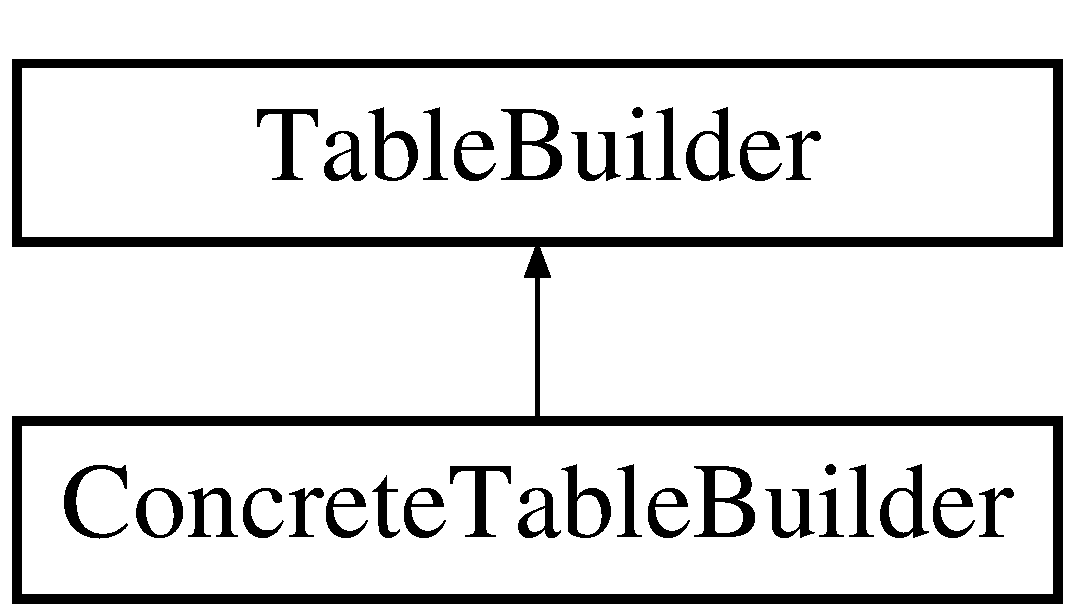
\includegraphics[height=2.000000cm]{class_table_builder}
\end{center}
\end{figure}
\subsection*{Public Member Functions}
\begin{DoxyCompactItemize}
\item 
virtual void \mbox{\hyperlink{class_table_builder_a4aba0952fb1912f9ff7ca4cfb3085dd9}{build\+Table}} ()
\item 
virtual void \mbox{\hyperlink{class_table_builder_a4269a0b8c10cf6fcae0c8525bdb08ff0}{buil\+Width}} (int width)
\item 
virtual void \mbox{\hyperlink{class_table_builder_ad3e3bb11cd8f9eecd49ad6012e358d05}{build\+Height}} (int height)
\item 
virtual void \mbox{\hyperlink{class_table_builder_a43bfcc7fbc5c45c0e2fe579b7d7e5f9c}{build\+Background\+Color}} (Q\+String color)
\item 
virtual void \mbox{\hyperlink{class_table_builder_a02a8d4ae71a3ef43ffd283ac10aa2e19}{build\+Friction}} (double friction)
\end{DoxyCompactItemize}


\subsection{Detailed Description}
Tablebuilder class is the abstract builder class for object table. 

\begin{DoxyAuthor}{Author}
Archibald Weng 
\end{DoxyAuthor}
\begin{DoxyDate}{Date}
April 2018 
\end{DoxyDate}


\subsection{Member Function Documentation}
\mbox{\Hypertarget{class_table_builder_a43bfcc7fbc5c45c0e2fe579b7d7e5f9c}\label{class_table_builder_a43bfcc7fbc5c45c0e2fe579b7d7e5f9c}} 
\index{Table\+Builder@{Table\+Builder}!build\+Background\+Color@{build\+Background\+Color}}
\index{build\+Background\+Color@{build\+Background\+Color}!Table\+Builder@{Table\+Builder}}
\subsubsection{\texorpdfstring{build\+Background\+Color()}{buildBackgroundColor()}}
{\footnotesize\ttfamily virtual void Table\+Builder\+::build\+Background\+Color (\begin{DoxyParamCaption}\item[{Q\+String}]{color }\end{DoxyParamCaption})\hspace{0.3cm}{\ttfamily [inline]}, {\ttfamily [virtual]}}

set the table\textquotesingle{}scolor 

Reimplemented in \mbox{\hyperlink{class_concrete_table_builder_a547c26af597d109dbaf9b4de32f041a9}{Concrete\+Table\+Builder}}.

\mbox{\Hypertarget{class_table_builder_a02a8d4ae71a3ef43ffd283ac10aa2e19}\label{class_table_builder_a02a8d4ae71a3ef43ffd283ac10aa2e19}} 
\index{Table\+Builder@{Table\+Builder}!build\+Friction@{build\+Friction}}
\index{build\+Friction@{build\+Friction}!Table\+Builder@{Table\+Builder}}
\subsubsection{\texorpdfstring{build\+Friction()}{buildFriction()}}
{\footnotesize\ttfamily virtual void Table\+Builder\+::build\+Friction (\begin{DoxyParamCaption}\item[{double}]{friction }\end{DoxyParamCaption})\hspace{0.3cm}{\ttfamily [inline]}, {\ttfamily [virtual]}}

set the table\textquotesingle{}s friction 

Reimplemented in \mbox{\hyperlink{class_concrete_table_builder_aab2c2ff234def292f7ead072dd5fda60}{Concrete\+Table\+Builder}}.

\mbox{\Hypertarget{class_table_builder_ad3e3bb11cd8f9eecd49ad6012e358d05}\label{class_table_builder_ad3e3bb11cd8f9eecd49ad6012e358d05}} 
\index{Table\+Builder@{Table\+Builder}!build\+Height@{build\+Height}}
\index{build\+Height@{build\+Height}!Table\+Builder@{Table\+Builder}}
\subsubsection{\texorpdfstring{build\+Height()}{buildHeight()}}
{\footnotesize\ttfamily virtual void Table\+Builder\+::build\+Height (\begin{DoxyParamCaption}\item[{int}]{height }\end{DoxyParamCaption})\hspace{0.3cm}{\ttfamily [inline]}, {\ttfamily [virtual]}}

set the table\textquotesingle{}s height 

Reimplemented in \mbox{\hyperlink{class_concrete_table_builder_a3e72d6d46e47146e385fff3937718a13}{Concrete\+Table\+Builder}}.

\mbox{\Hypertarget{class_table_builder_a4aba0952fb1912f9ff7ca4cfb3085dd9}\label{class_table_builder_a4aba0952fb1912f9ff7ca4cfb3085dd9}} 
\index{Table\+Builder@{Table\+Builder}!build\+Table@{build\+Table}}
\index{build\+Table@{build\+Table}!Table\+Builder@{Table\+Builder}}
\subsubsection{\texorpdfstring{build\+Table()}{buildTable()}}
{\footnotesize\ttfamily virtual void Table\+Builder\+::build\+Table (\begin{DoxyParamCaption}{ }\end{DoxyParamCaption})\hspace{0.3cm}{\ttfamily [inline]}, {\ttfamily [virtual]}}

build a table 

Reimplemented in \mbox{\hyperlink{class_concrete_table_builder_af49b5e371e6f725303e4b2f011d20fad}{Concrete\+Table\+Builder}}.

\mbox{\Hypertarget{class_table_builder_a4269a0b8c10cf6fcae0c8525bdb08ff0}\label{class_table_builder_a4269a0b8c10cf6fcae0c8525bdb08ff0}} 
\index{Table\+Builder@{Table\+Builder}!buil\+Width@{buil\+Width}}
\index{buil\+Width@{buil\+Width}!Table\+Builder@{Table\+Builder}}
\subsubsection{\texorpdfstring{buil\+Width()}{builWidth()}}
{\footnotesize\ttfamily virtual void Table\+Builder\+::buil\+Width (\begin{DoxyParamCaption}\item[{int}]{width }\end{DoxyParamCaption})\hspace{0.3cm}{\ttfamily [inline]}, {\ttfamily [virtual]}}

set the table\textquotesingle{}s width 

The documentation for this class was generated from the following files\+:\begin{DoxyCompactItemize}
\item 
tablebuilder.\+h\item 
tablebuilder.\+cpp\end{DoxyCompactItemize}

%--- End generated contents ---

% Index
\backmatter
\newpage
\phantomsection
\clearemptydoublepage
\addcontentsline{toc}{chapter}{Index}
\printindex

\end{document}
